\chapter{Project 4: Sensor}

\section{Overview}
Now that you have a handle on how to work with LEDs and buttons, let's look at something a little more complex.
This project will introduce a humidity and temperature sensor. Over the course of this project, you will:
\begin{itemize}
    \item Connect a sensor board to your microcontroller
    \item Import a library into your code that knows how to communicate with that sensor
    \item Use MicroPython to poll the sensor over and over to write out the current result
    \item Connect a screen to your microcontroller and output the sensor data to it
\end{itemize}
At the end of this project, your microcontroller should run a MicroPython program that prints out the current
temperature and humidity of the room you're sitting in. Let's get started!
\begin{figure}[H]
\centering
    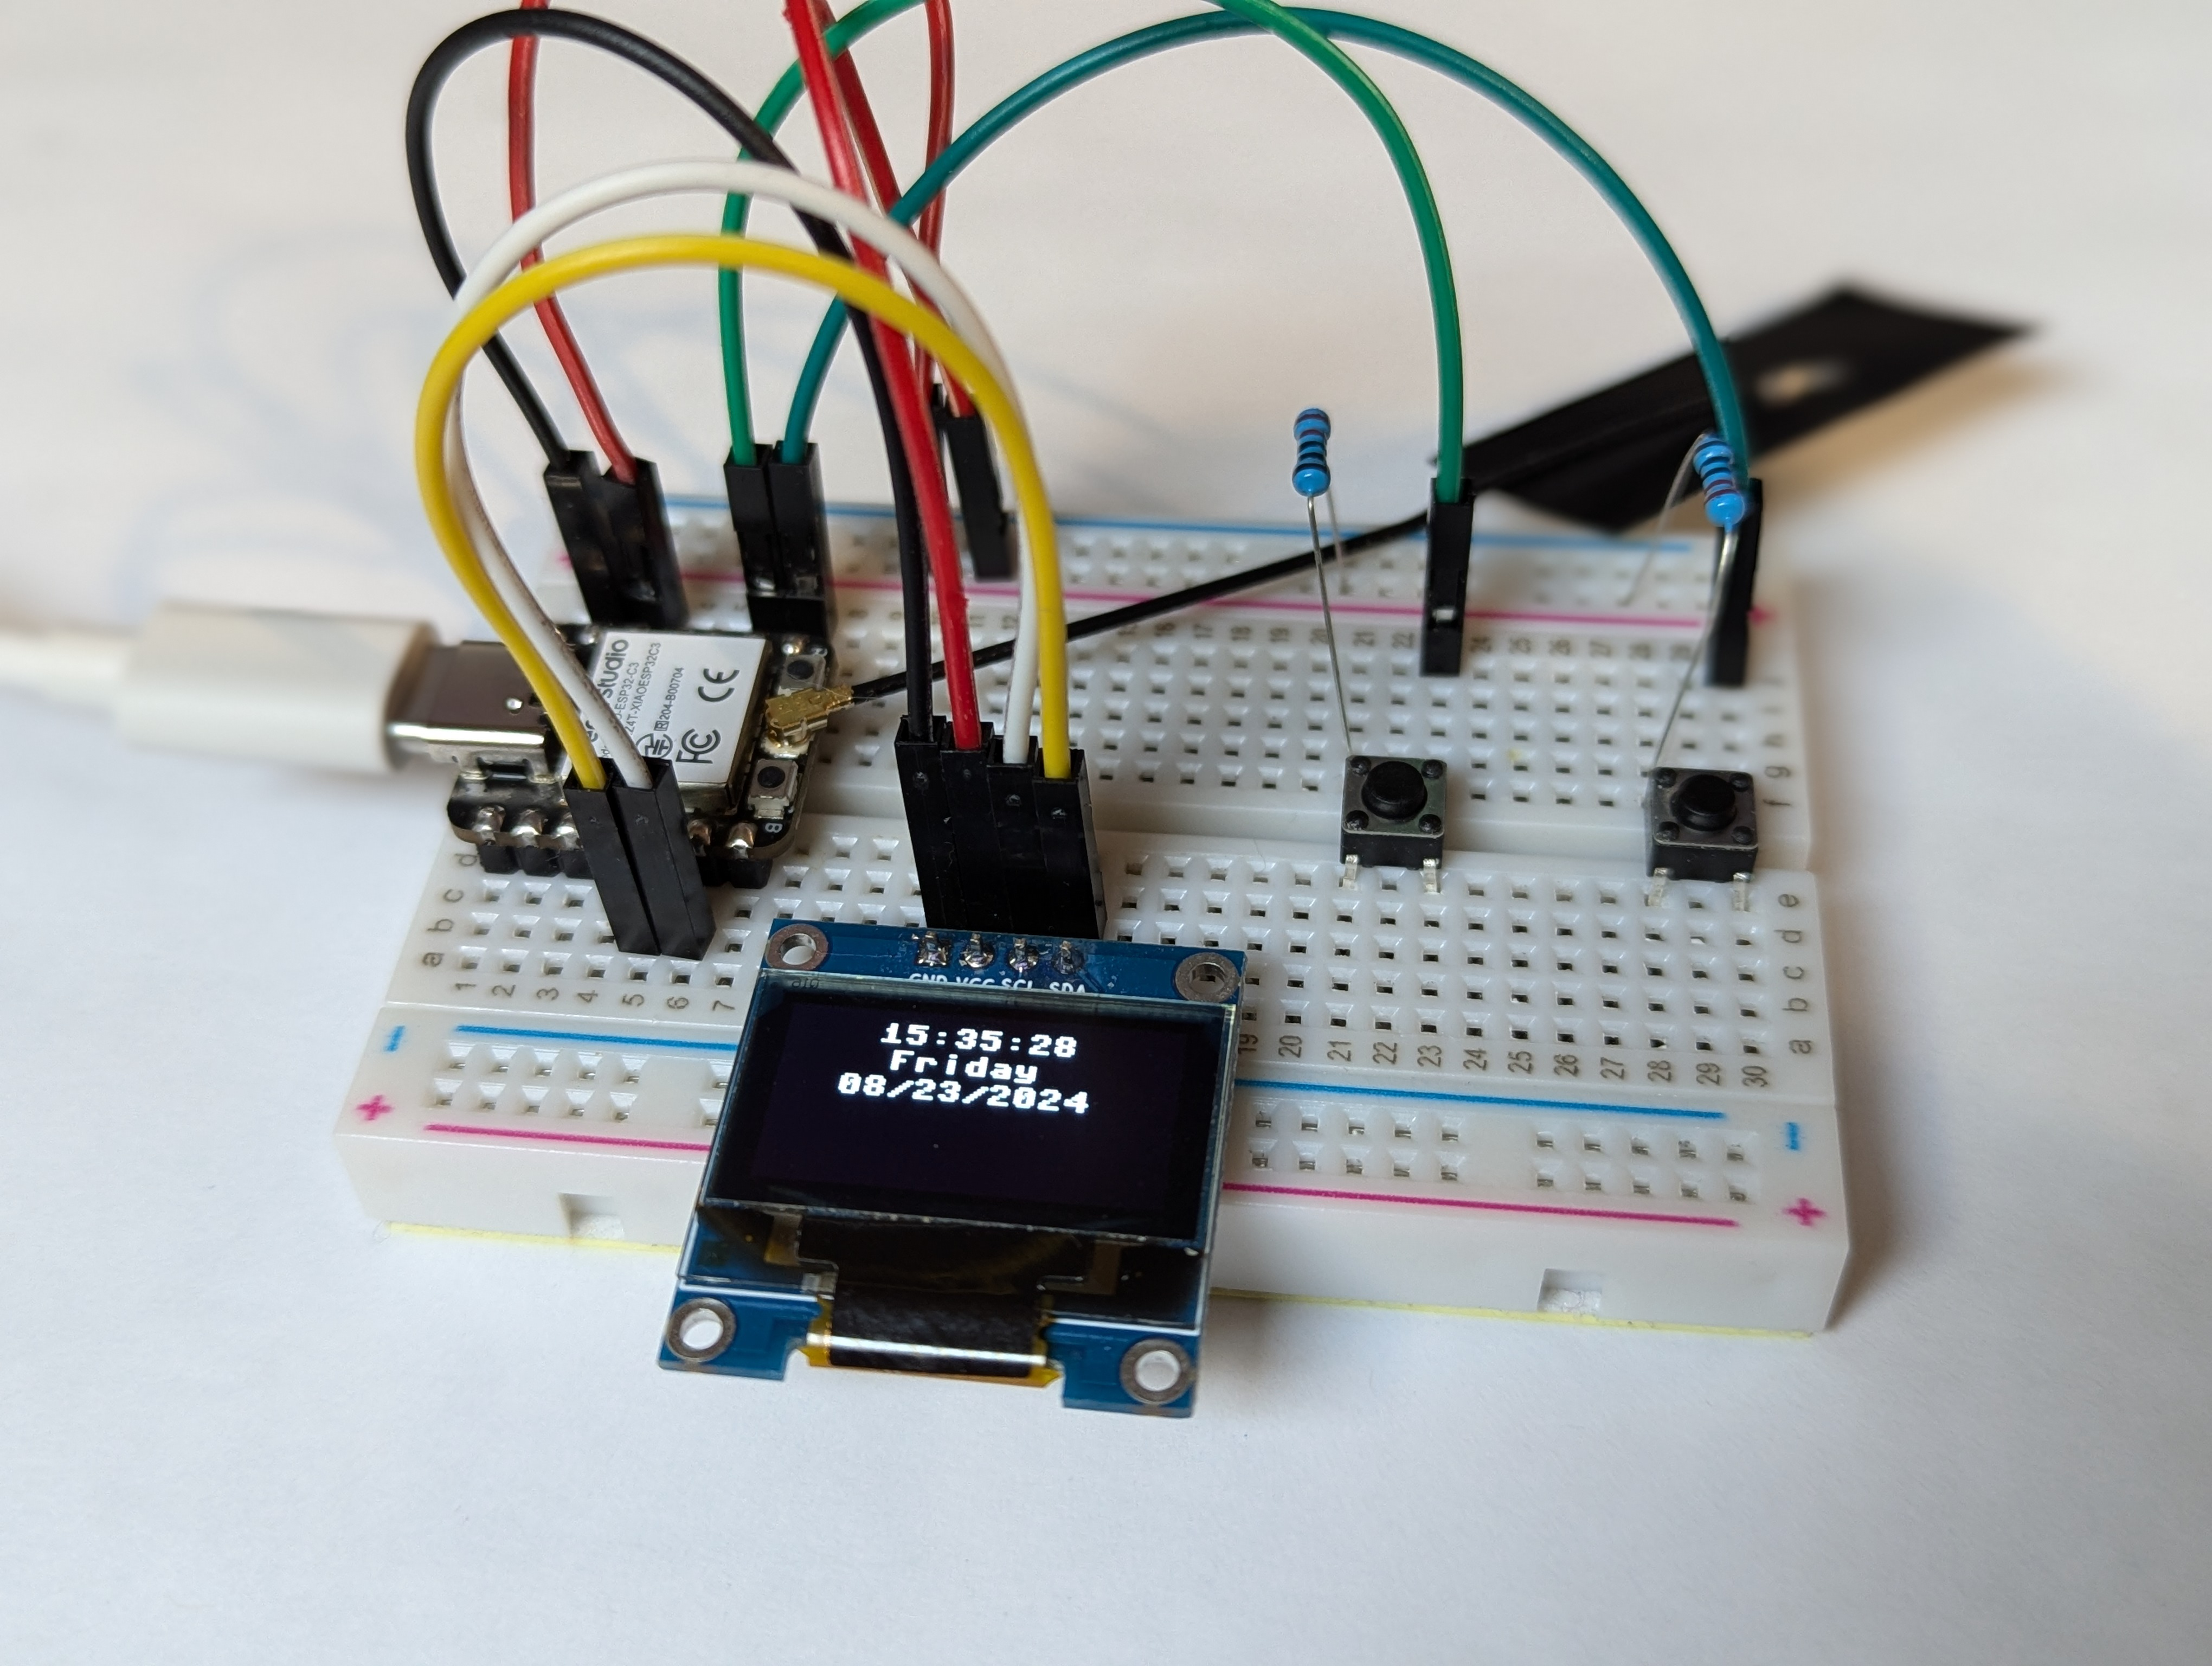
\includegraphics[width=.6\linewidth]{project_4/screen_connected.jpg}
    \caption{The end result should look something like this}
\end{figure}

\pagebreak

\section{Directions}

\subsection{Creating the circuit}
Using jumper cables, you will be assembling a circuit between your microcontroller, your breadboard, and the small
temperature/humidity board included in your kit.

\subsubsection{Remove previous components}
Before beginning, remove any components from prior chapters including LEDs, buttons, and wires. You may leave the
microcontroller attached to the breadboard.

\subsubsection{Attach the microcontroller to the breadboard}
If it's not already, carefully insert the pins at the bottom of your microcontroller into the breadboard. Refer back
to \ref{pinout} for pin labels. When placing the board into the breadboard, make sure that the microcontroller is oriented such that:
\begin{itemize}
    \item The pin labeled \textbf{5V} is inserted in hole at \textbf{Column H, Row 1} of the breadboard (or \textbf{H1}, for short)
    \item The pin labeled \textbf{GPIO2} is inserted in hole \textbf{D1} of the breadboard
    \item The pin labeled \textbf{GPIO20} is inserted in hole \textbf{H7} of the breadboard
    \item the pin labeled \textbf{GPIO21} is inserted in hole \textbf{D7} of the breadboard
\end{itemize}
You may need to apply more pressure than expected to seat the microcontroller properly in the breadboard. When its over, it should look like this:
\begin{figure}[H]
    \centering
    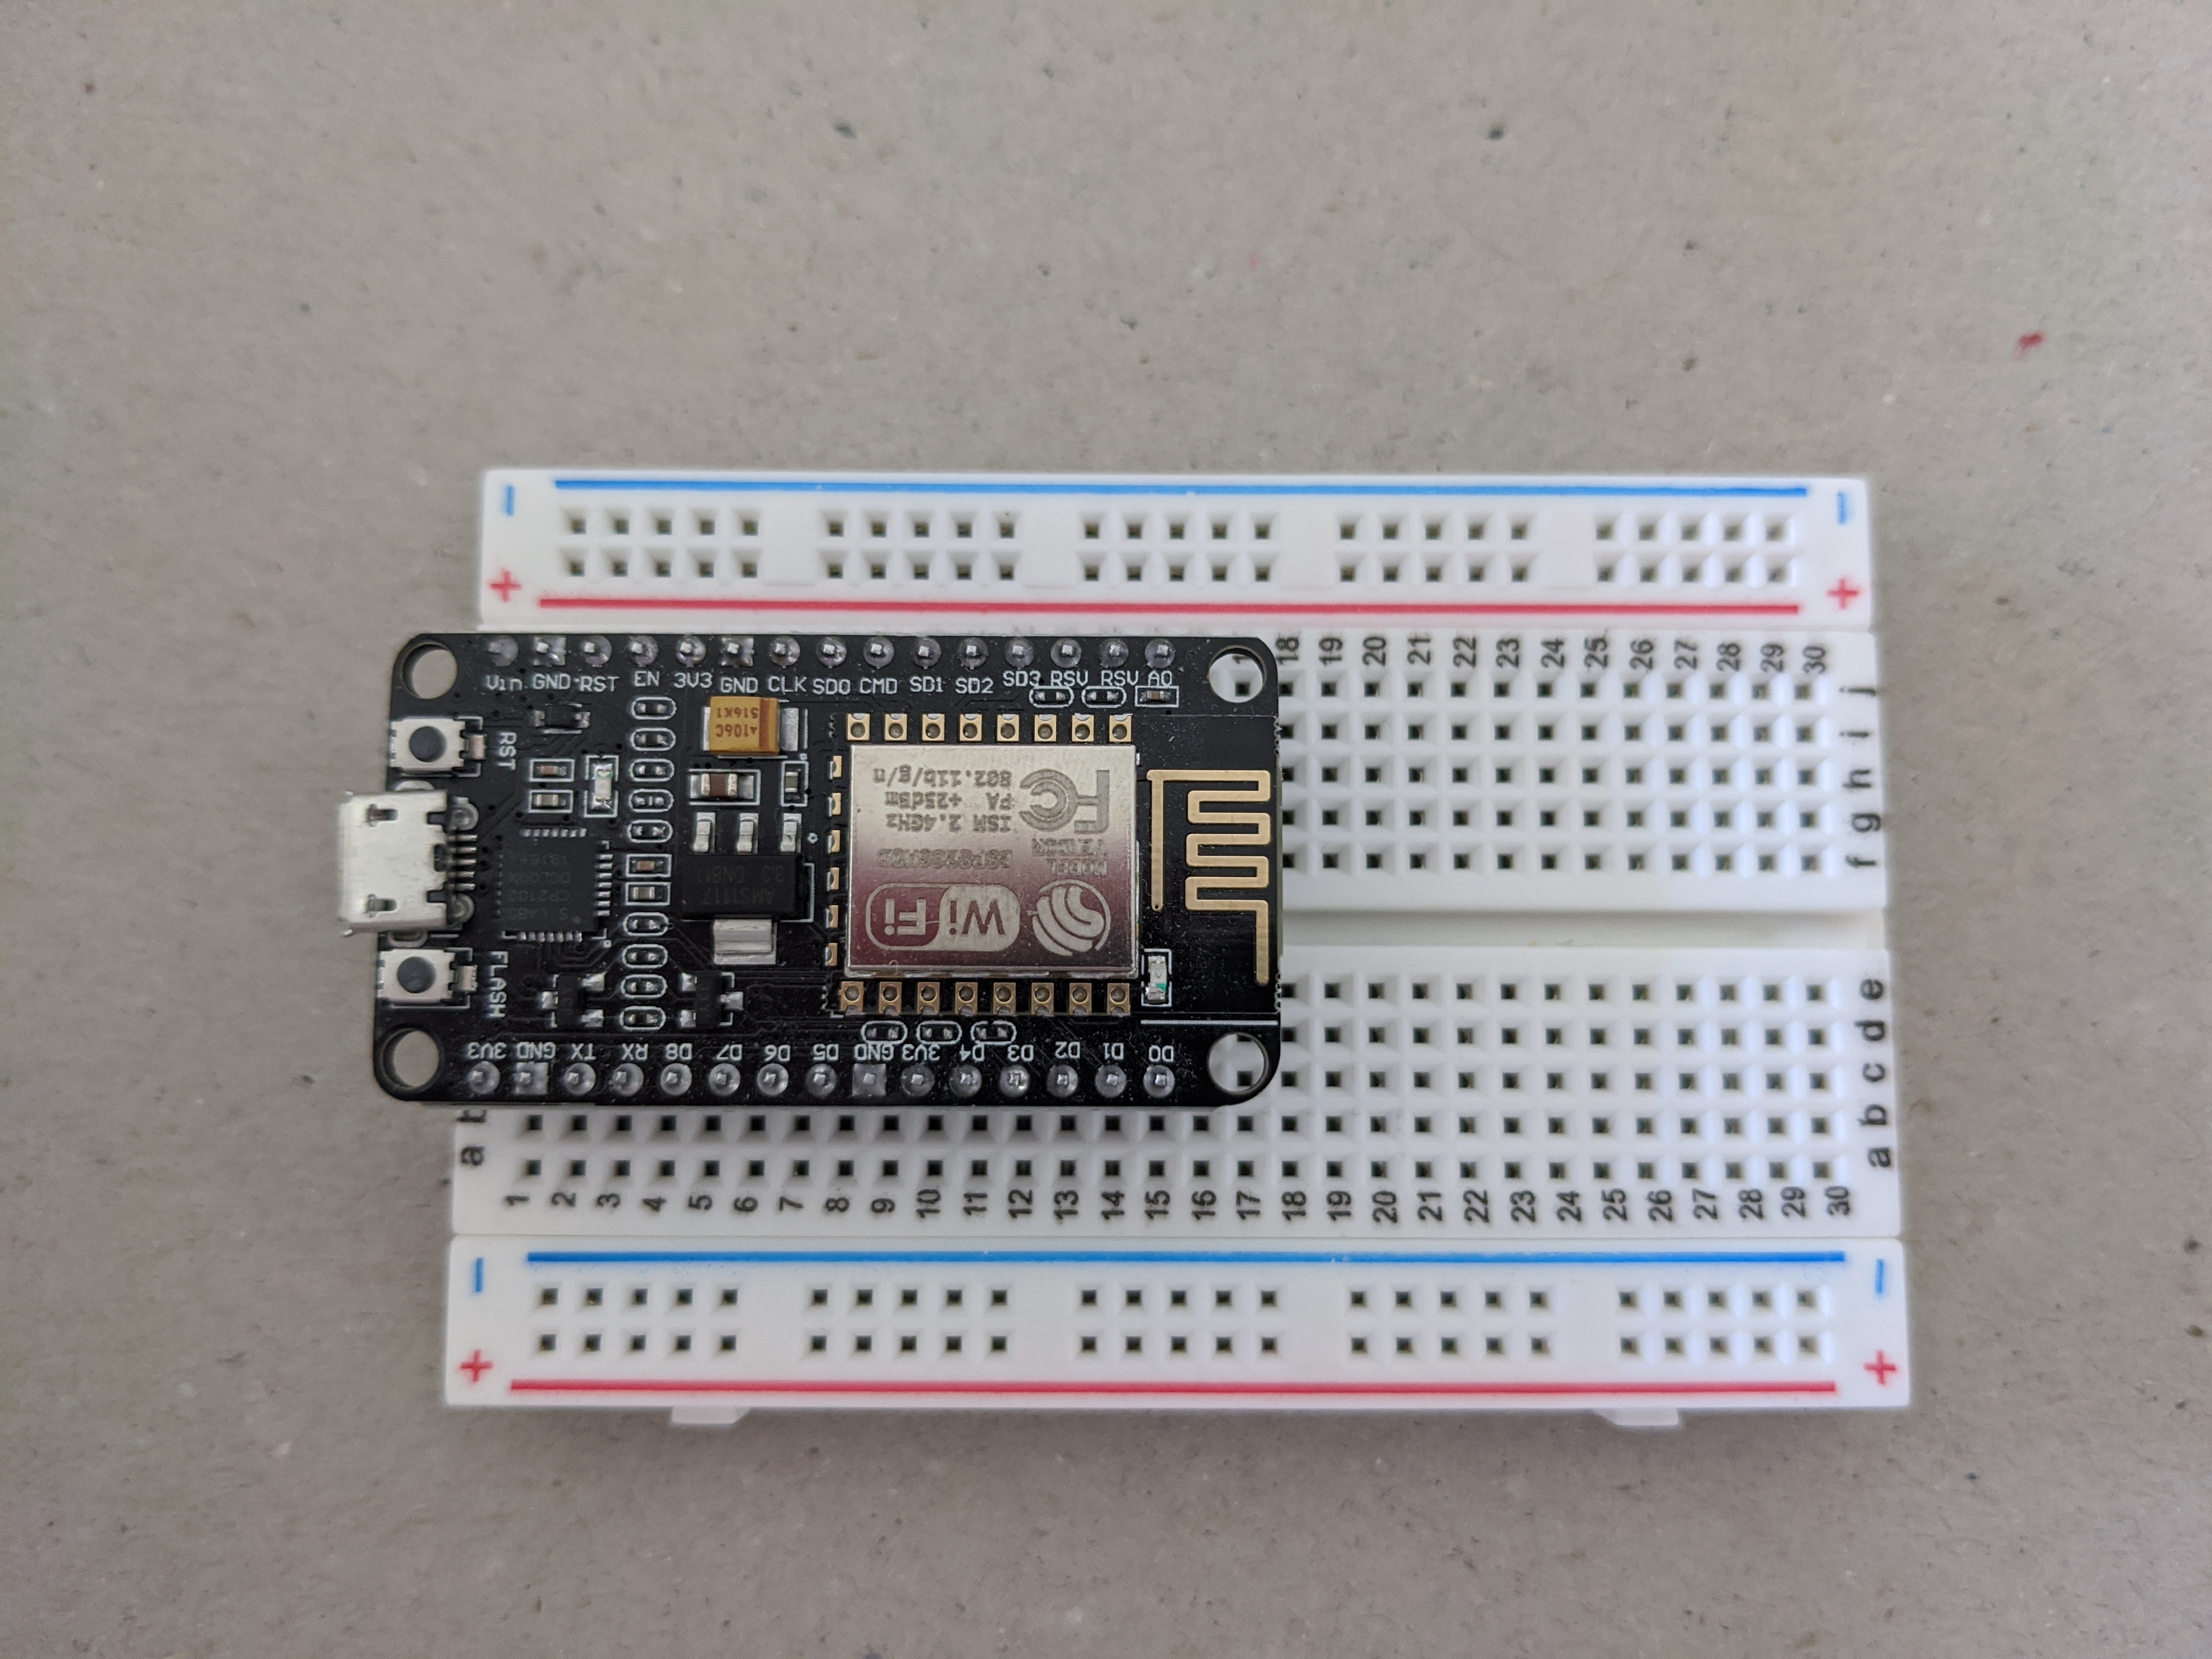
\includegraphics[width=.6\linewidth]{common/microcontroller_seated_in_breadboard.jpg}
    \caption{So far, so good!}
\end{figure}

\subsubsection{Connect the necessary jumper wires}
\begin{itemize}
    \item Place a red jumper wire into hole \textbf{J3} of the breadboard and the other end in
    hole \textbf{D16} of the breadboard. This will provide \textbf{3.3} volts of power to the temperature/humidity sensor.
    \item Place a black jumper wire into hole \textbf{J2} of the breadboard and the other
    end in hole \textbf{D17} of the breadboard. This will provide the ground connection for the temperature/humidity sensor.
    \item Place a white jumper wire into hole \textbf{B6} of the breadboard and the other
    end in hole \textbf{D18} of the breadboard. This will provide a clock signal to the sensor board.
    \item Plase a yellow jumper wire into hole \textbf{B5} of the breadboard and the other
    end in hole \textbf{D19} of the breadboard. This will transmit data from the sensor back to the microcontroller.
\end{itemize}

You should be left with something that looks like this:
\begin{figure}[H]
    \centering
    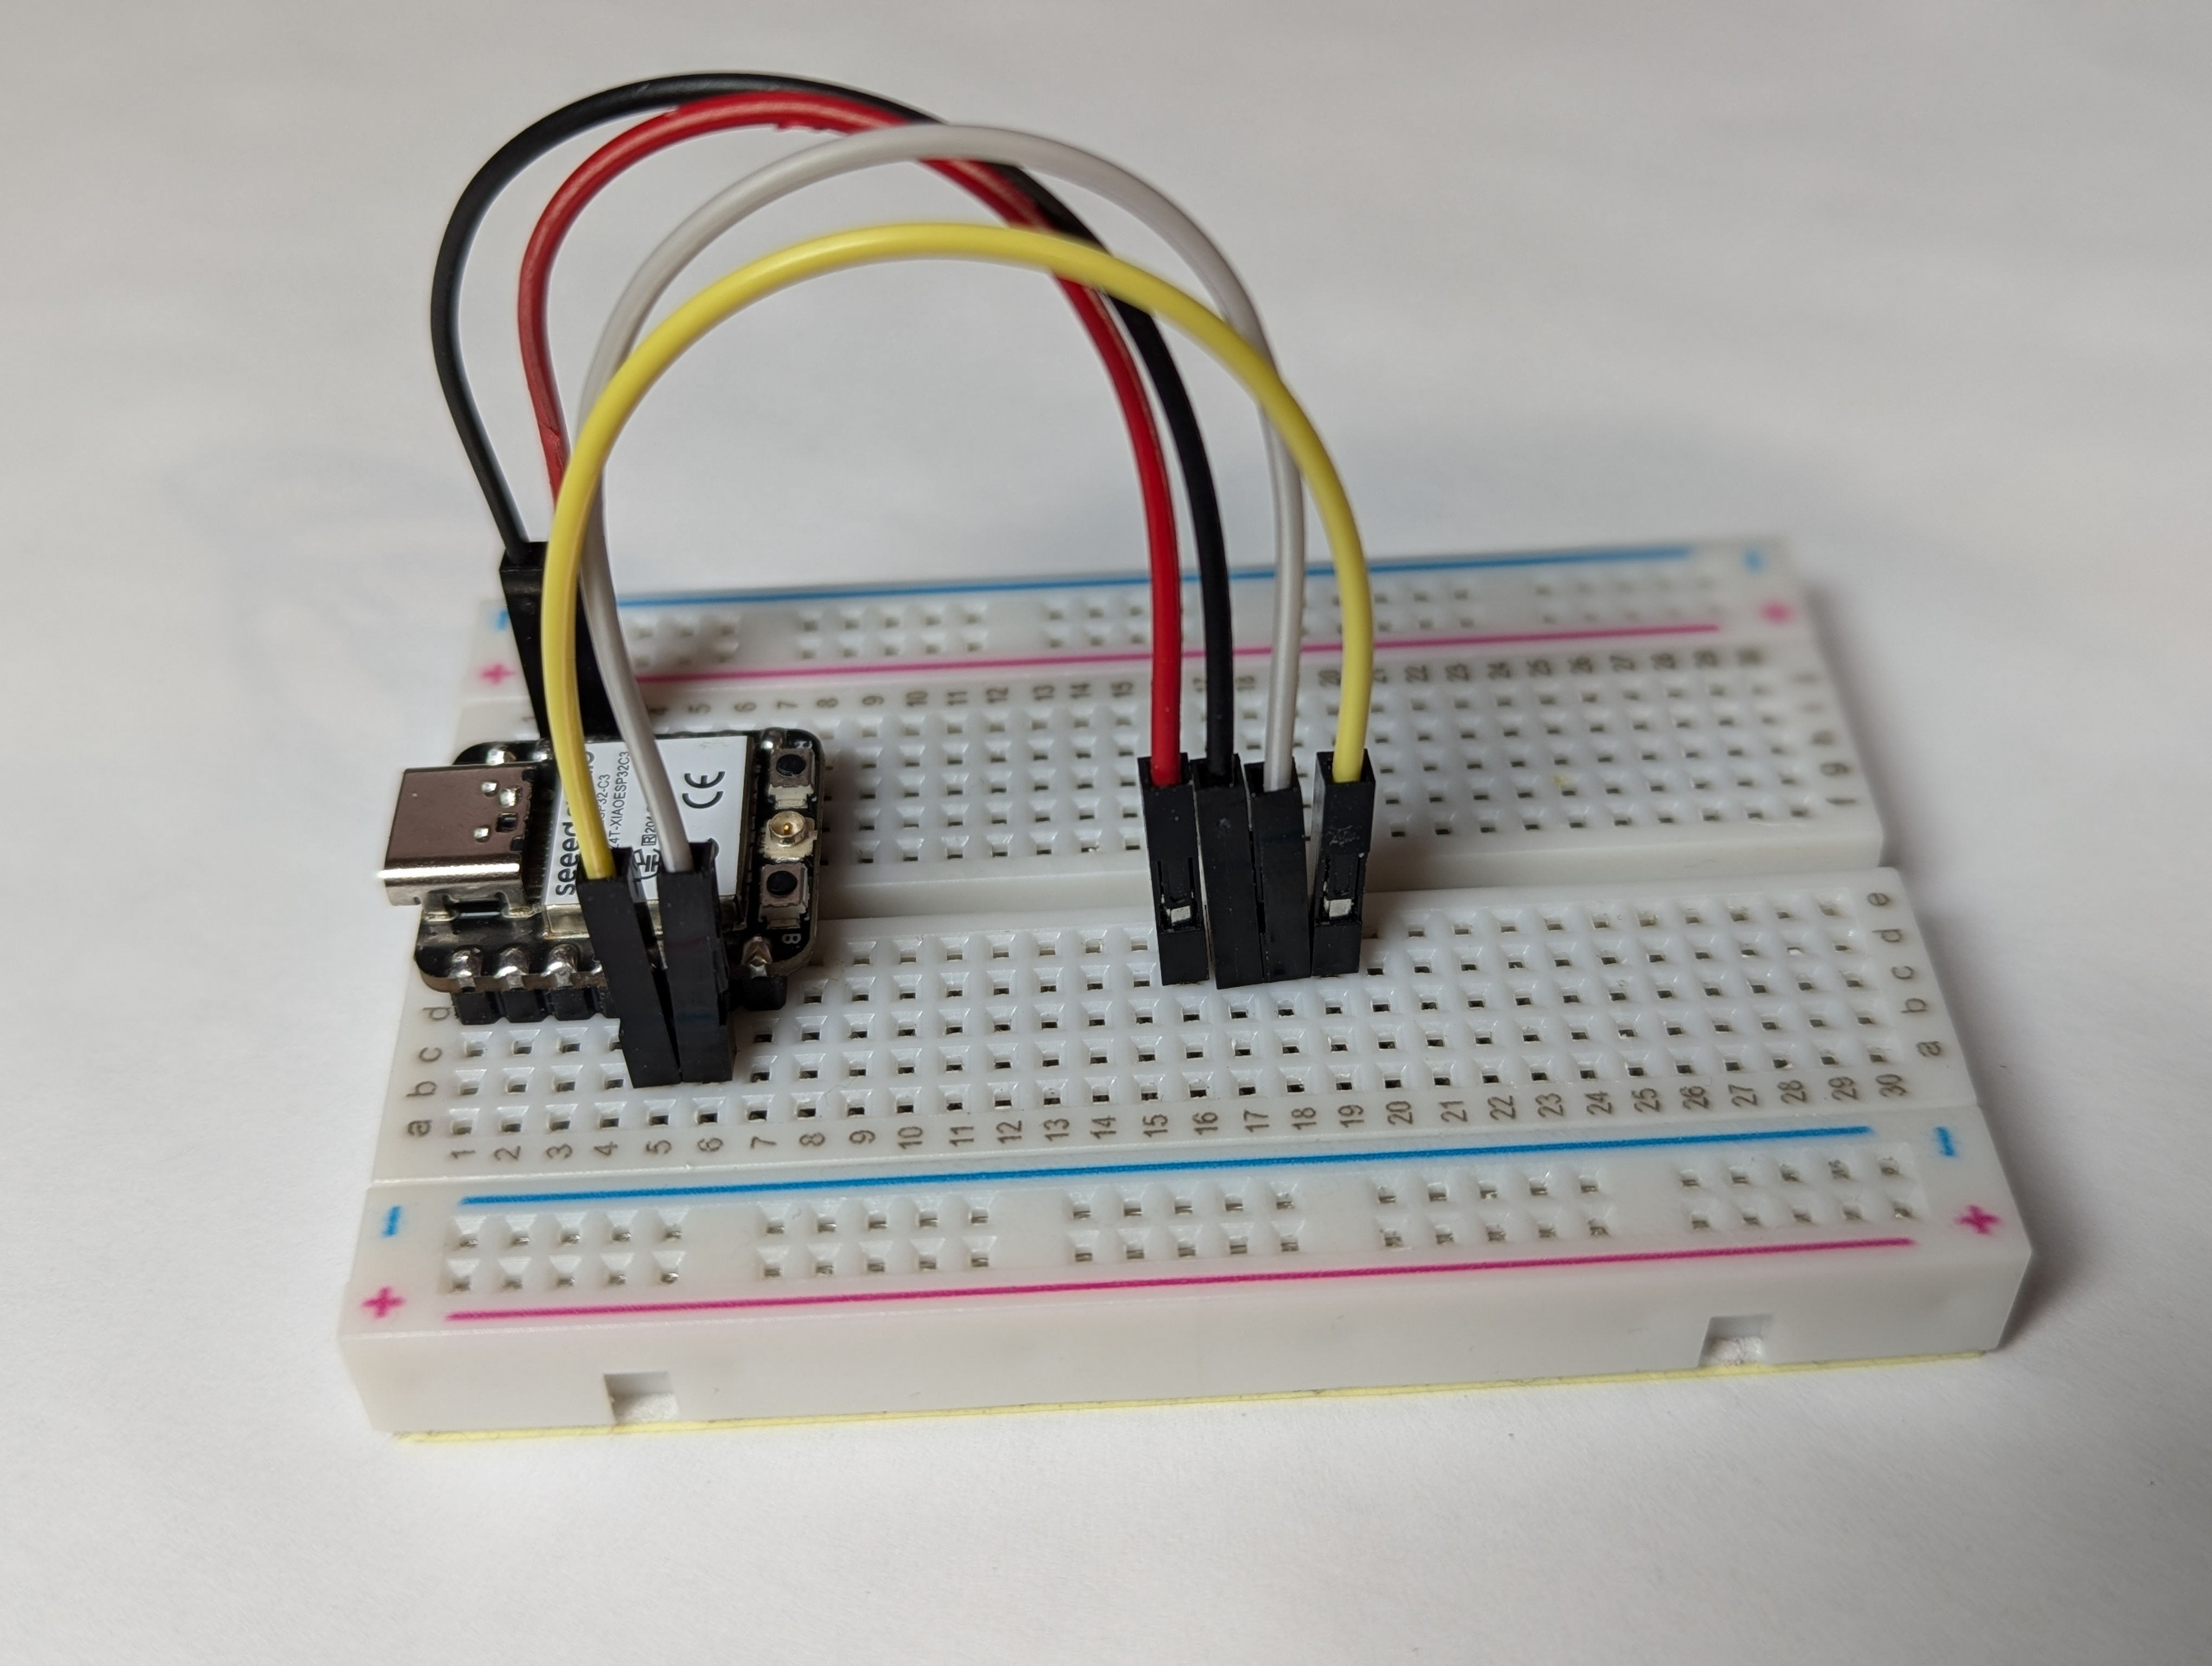
\includegraphics[width=.6\linewidth]{project_4/sensor_board_wired.jpg}
    \caption{There are 4 wires that will be connected between the microcontroller and the sensor board.}
\end{figure}

\subsubsection{Attach the temperature/humidity sensor to the breadboard}
Plug the 4 pins of the sensor board into the breadboard just under where the 4 jumper wires are lined up. Make sure the pins
of the board are lined up with the jumper wires and the board points away from them. It should look like this:

\begin{figure}[H]
    \centering
    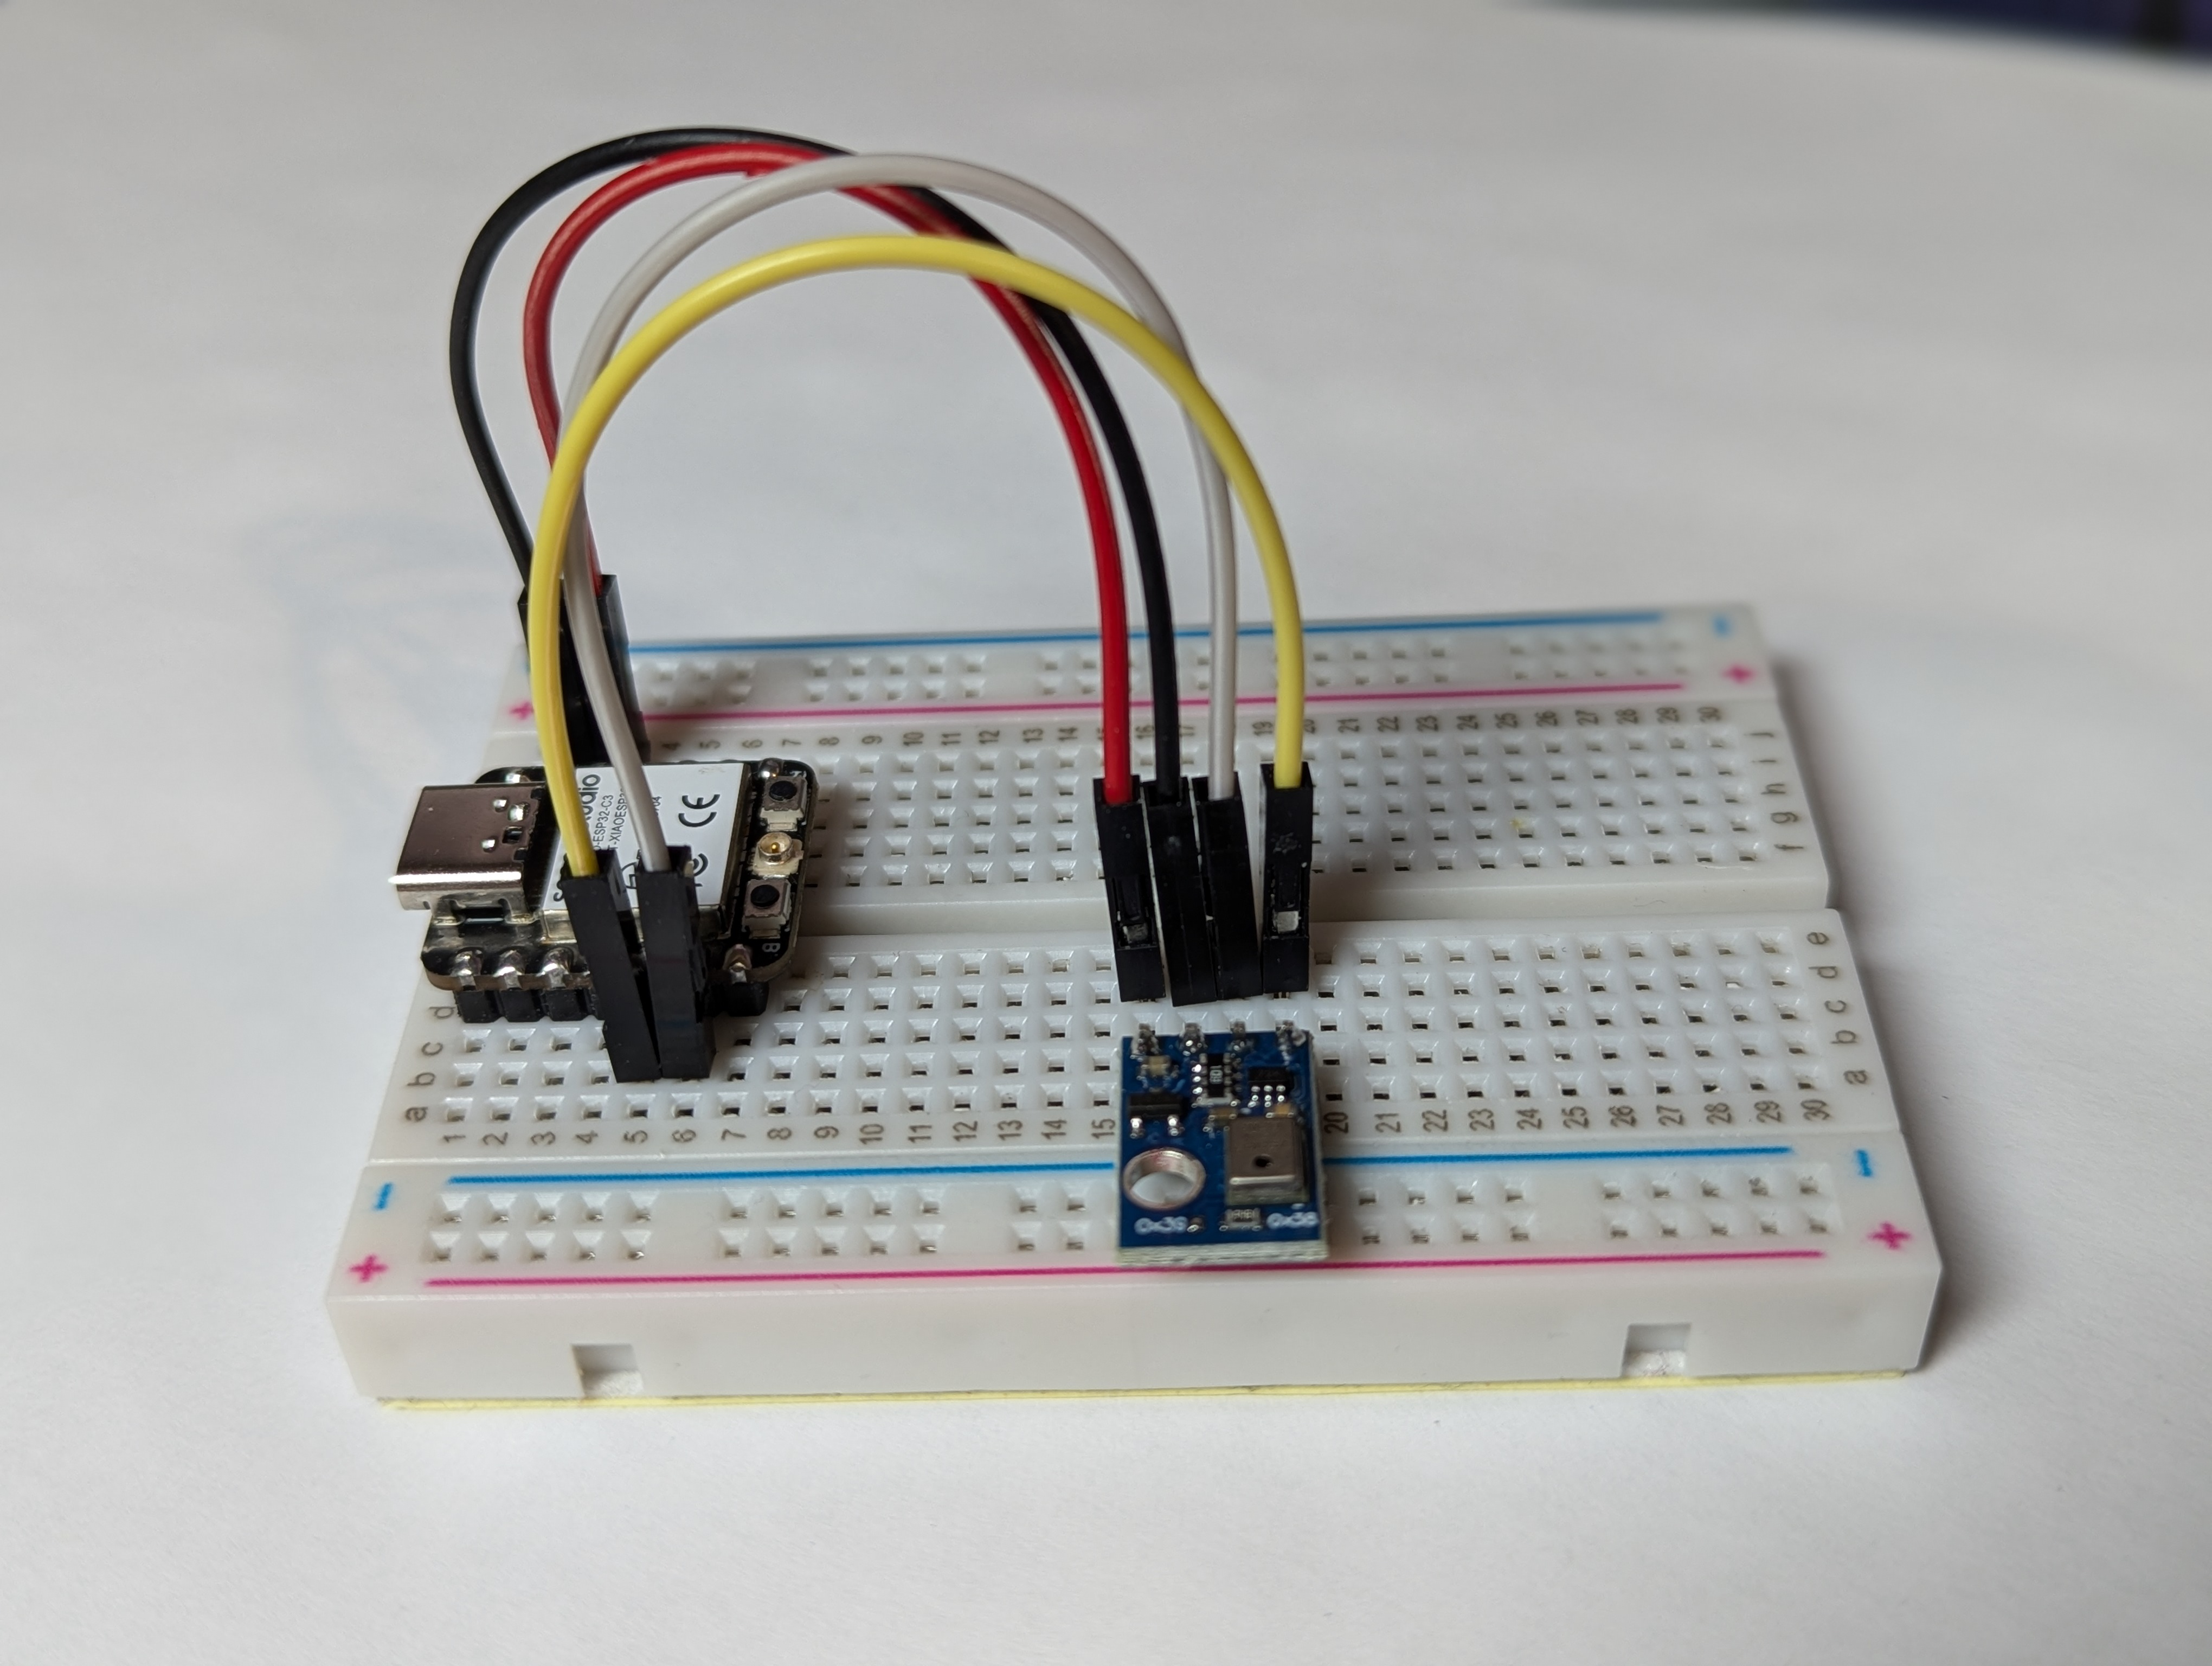
\includegraphics[width=.6\linewidth]{project_4/sensor_board_connected.jpg}
    \caption{Click the button highlighted in red.}
\end{figure}

\subsection{Programming the microcontroller}
Once all of the wiring is correct, connect the USB cable to the microcontroller and go to https://viper-ide.org/ in your
computer's web browser. Click on the USB icon in the top right and choose your microcontroller from the list:

\begin{figure}[H]
    \centering
    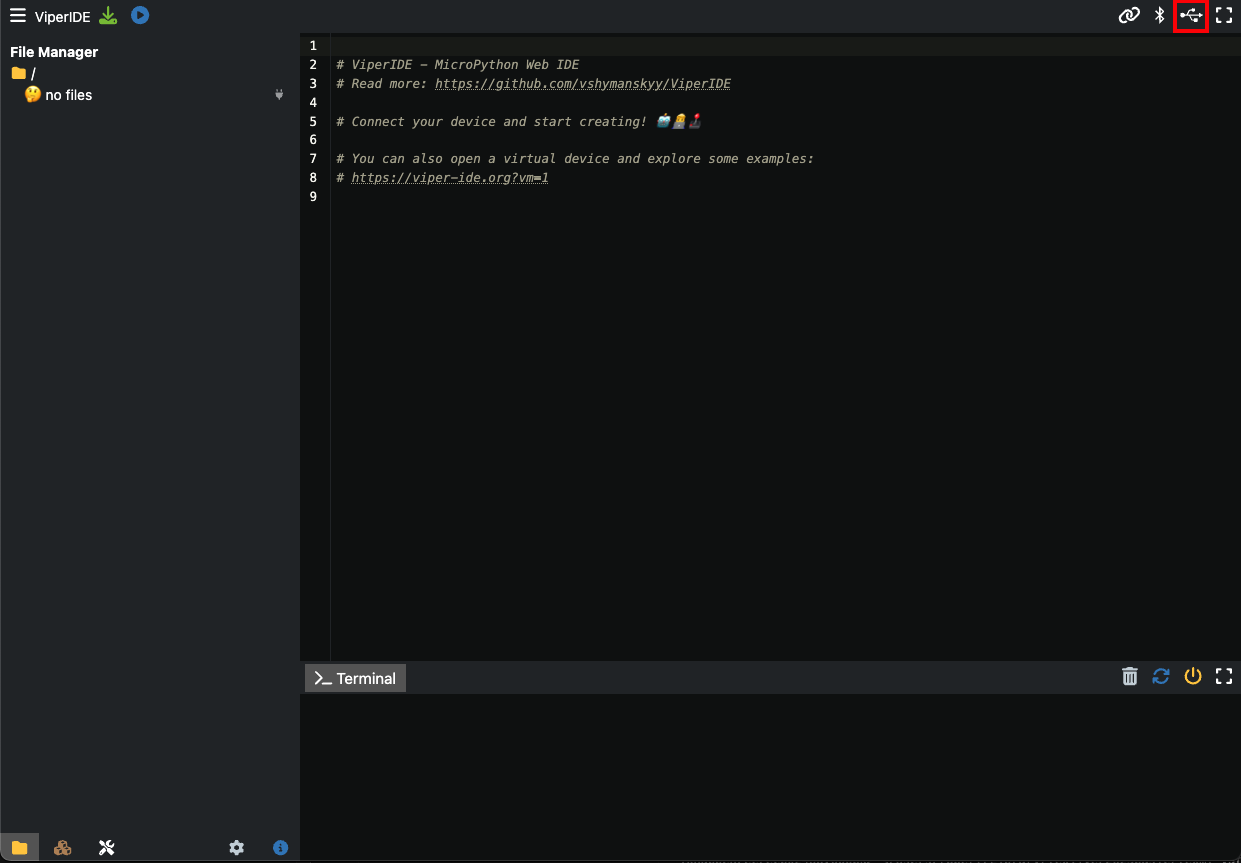
\includegraphics[width=.6\linewidth]{common/viper_ide_usb_connect.png}
    \caption{Click the button highlighted in red.}
\end{figure}

If you see multiple items in the dialog that pops up, choose the one that starts with "USB JTAG". See below for an example:
\begin{figure}[H]
    \centering
    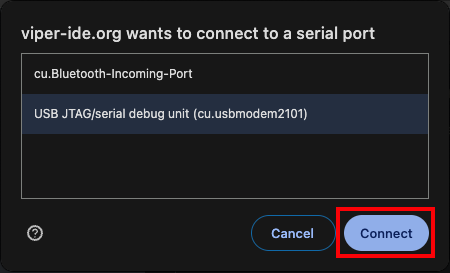
\includegraphics[width=.6\linewidth]{common/viper_ide_usb_choice_connect.png}
    \caption{Click the button highlighted in red.}
\end{figure}

Once you have connected, you will see a green dialog labeled "Device connected" and the file manager on the list
will populate with the list of files installed on the device:
\begin{figure}[H]
    \centering
    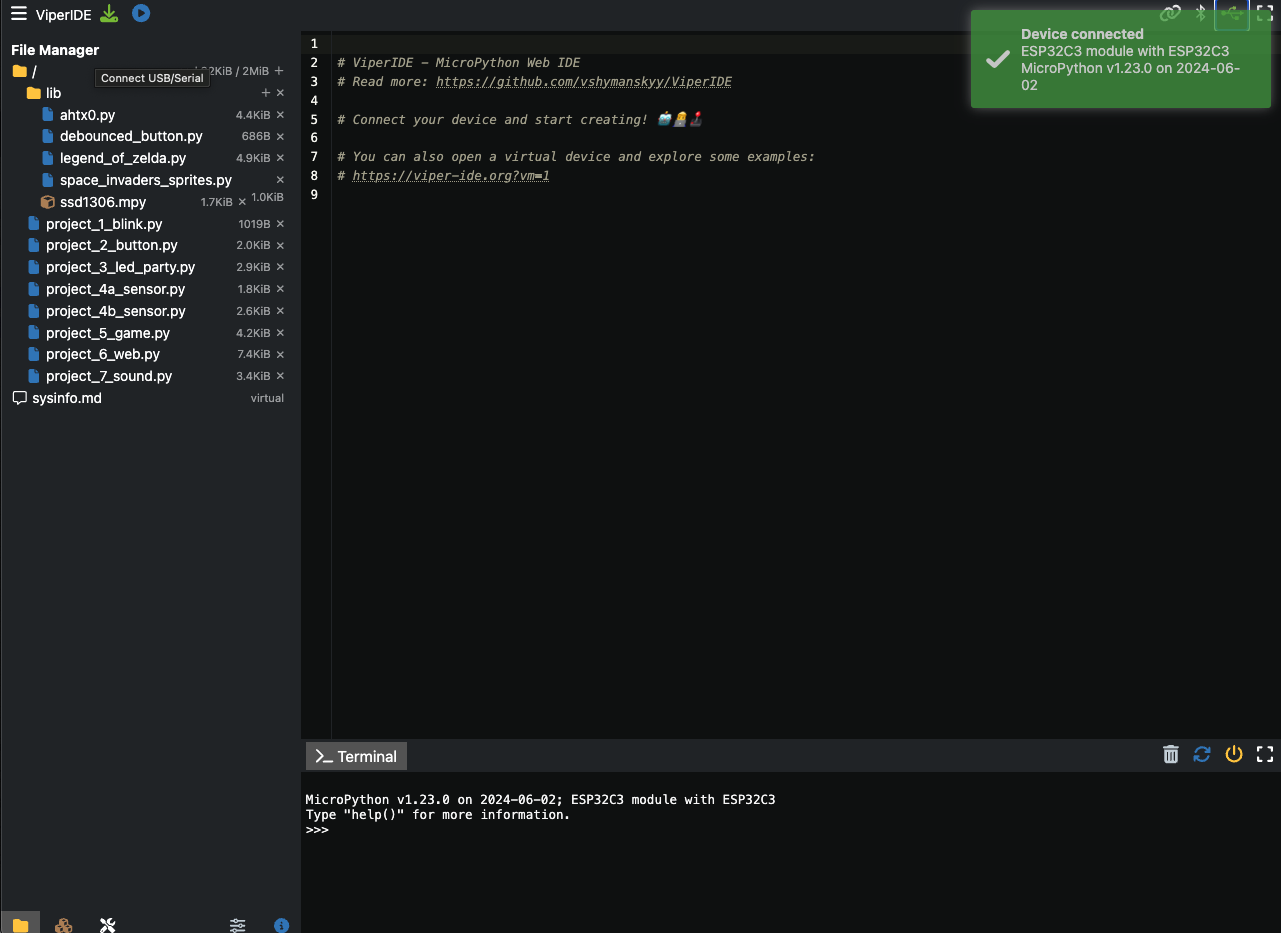
\includegraphics[width=.6\linewidth]{common/viper_connected.png}
    \caption{Make sure to open the right file for this project}
\end{figure}

Click on the file named "project\_4a\_sensor.py". This will load the code in the editor for this section. Read through the comments
and the code to get a sense for how it works. Once you are ready, you can click the blue play button in the upper left of the window to start the script:
\begin{figure}[H]
    \centering
    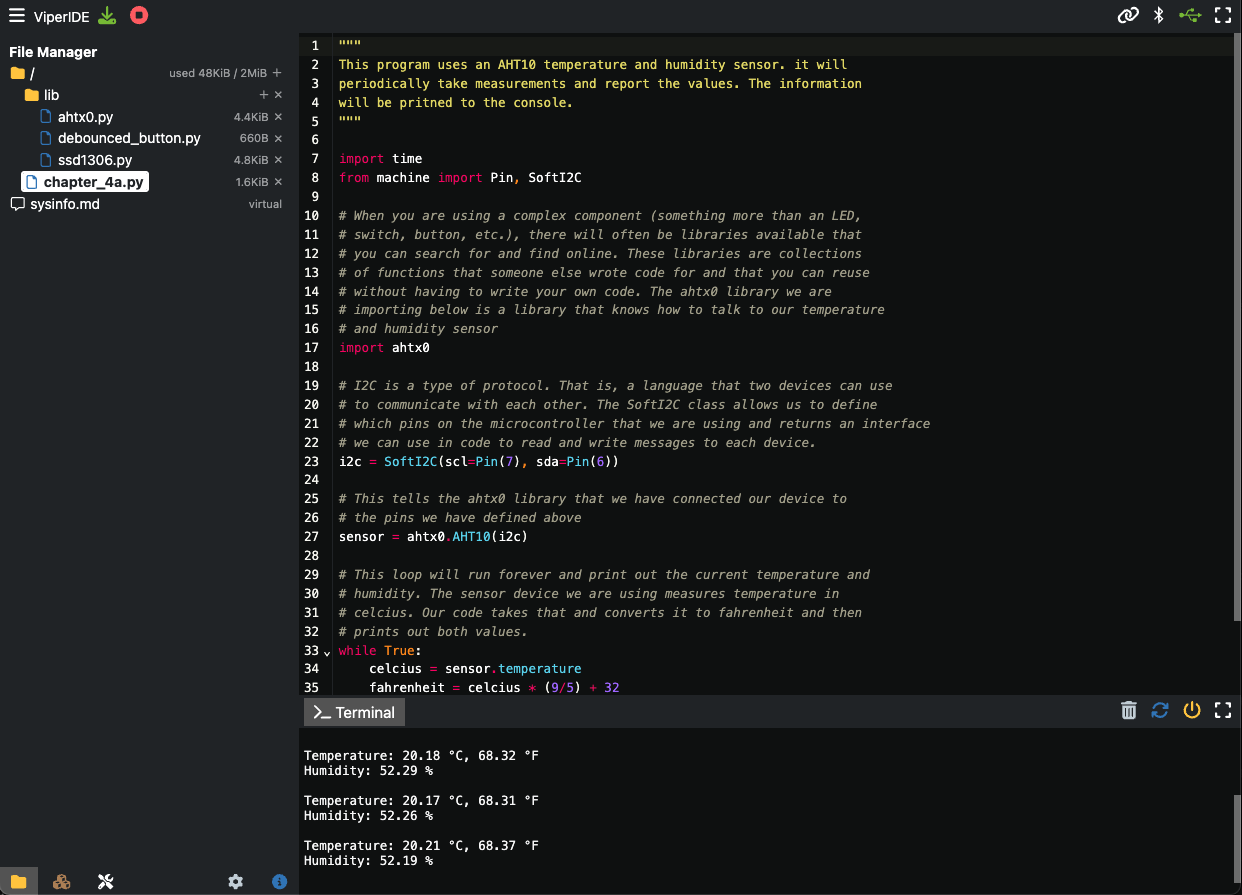
\includegraphics[width=.6\linewidth]{project_4/play_project_4a.png}
    \caption{Once started, this script will run forever and output values into the terminal window. You can stop by pressing the red stop button.}
\end{figure}

\subsection{Making it fancier}
Having the temperature and humidity print out to the terminal is pretty cool (or pretty warm depending on where you are).
But wouldn't it be better if we didn't have to be connected to a computer to see the values? We can give our device a screen and have it print the values out there as well.

\subsubsection{Connect the necessary jumper wires}
\begin{itemize}
    \item First, disconnect the USB cable from your microcontroller. Doing this prevents accidentally connecting power to somewhere it shouln't go!
    \item Place a red jumper wire into hole \textbf{E16} of the breadboard and the other end in
    hole \textbf{E25} of the breadboard. This will provide \textbf{3.3} volts of power to the screen.
    \item Place a black jumper wire into hole \textbf{E17} of the breadboard and the other end
    in hole \textbf{E24} of the breadboard. This will provide the ground connection for the screen.
    \item Place a white jumper wire into hole \textbf{E18} of the breadboard and the other end
    in hole \textbf{E26} of the breadboard. This will provide a clock signal to the screen.
    \item Place a yellow jumper wire into hole \textbf{B4} of the breadboard and the other
    end in hole \textbf{E27} of the breadboard. This will transmit data from the microcontroller to the screen to be displayed.
\end{itemize}

You should be left with something that looks like this:
\begin{figure}[H]
    \centering
    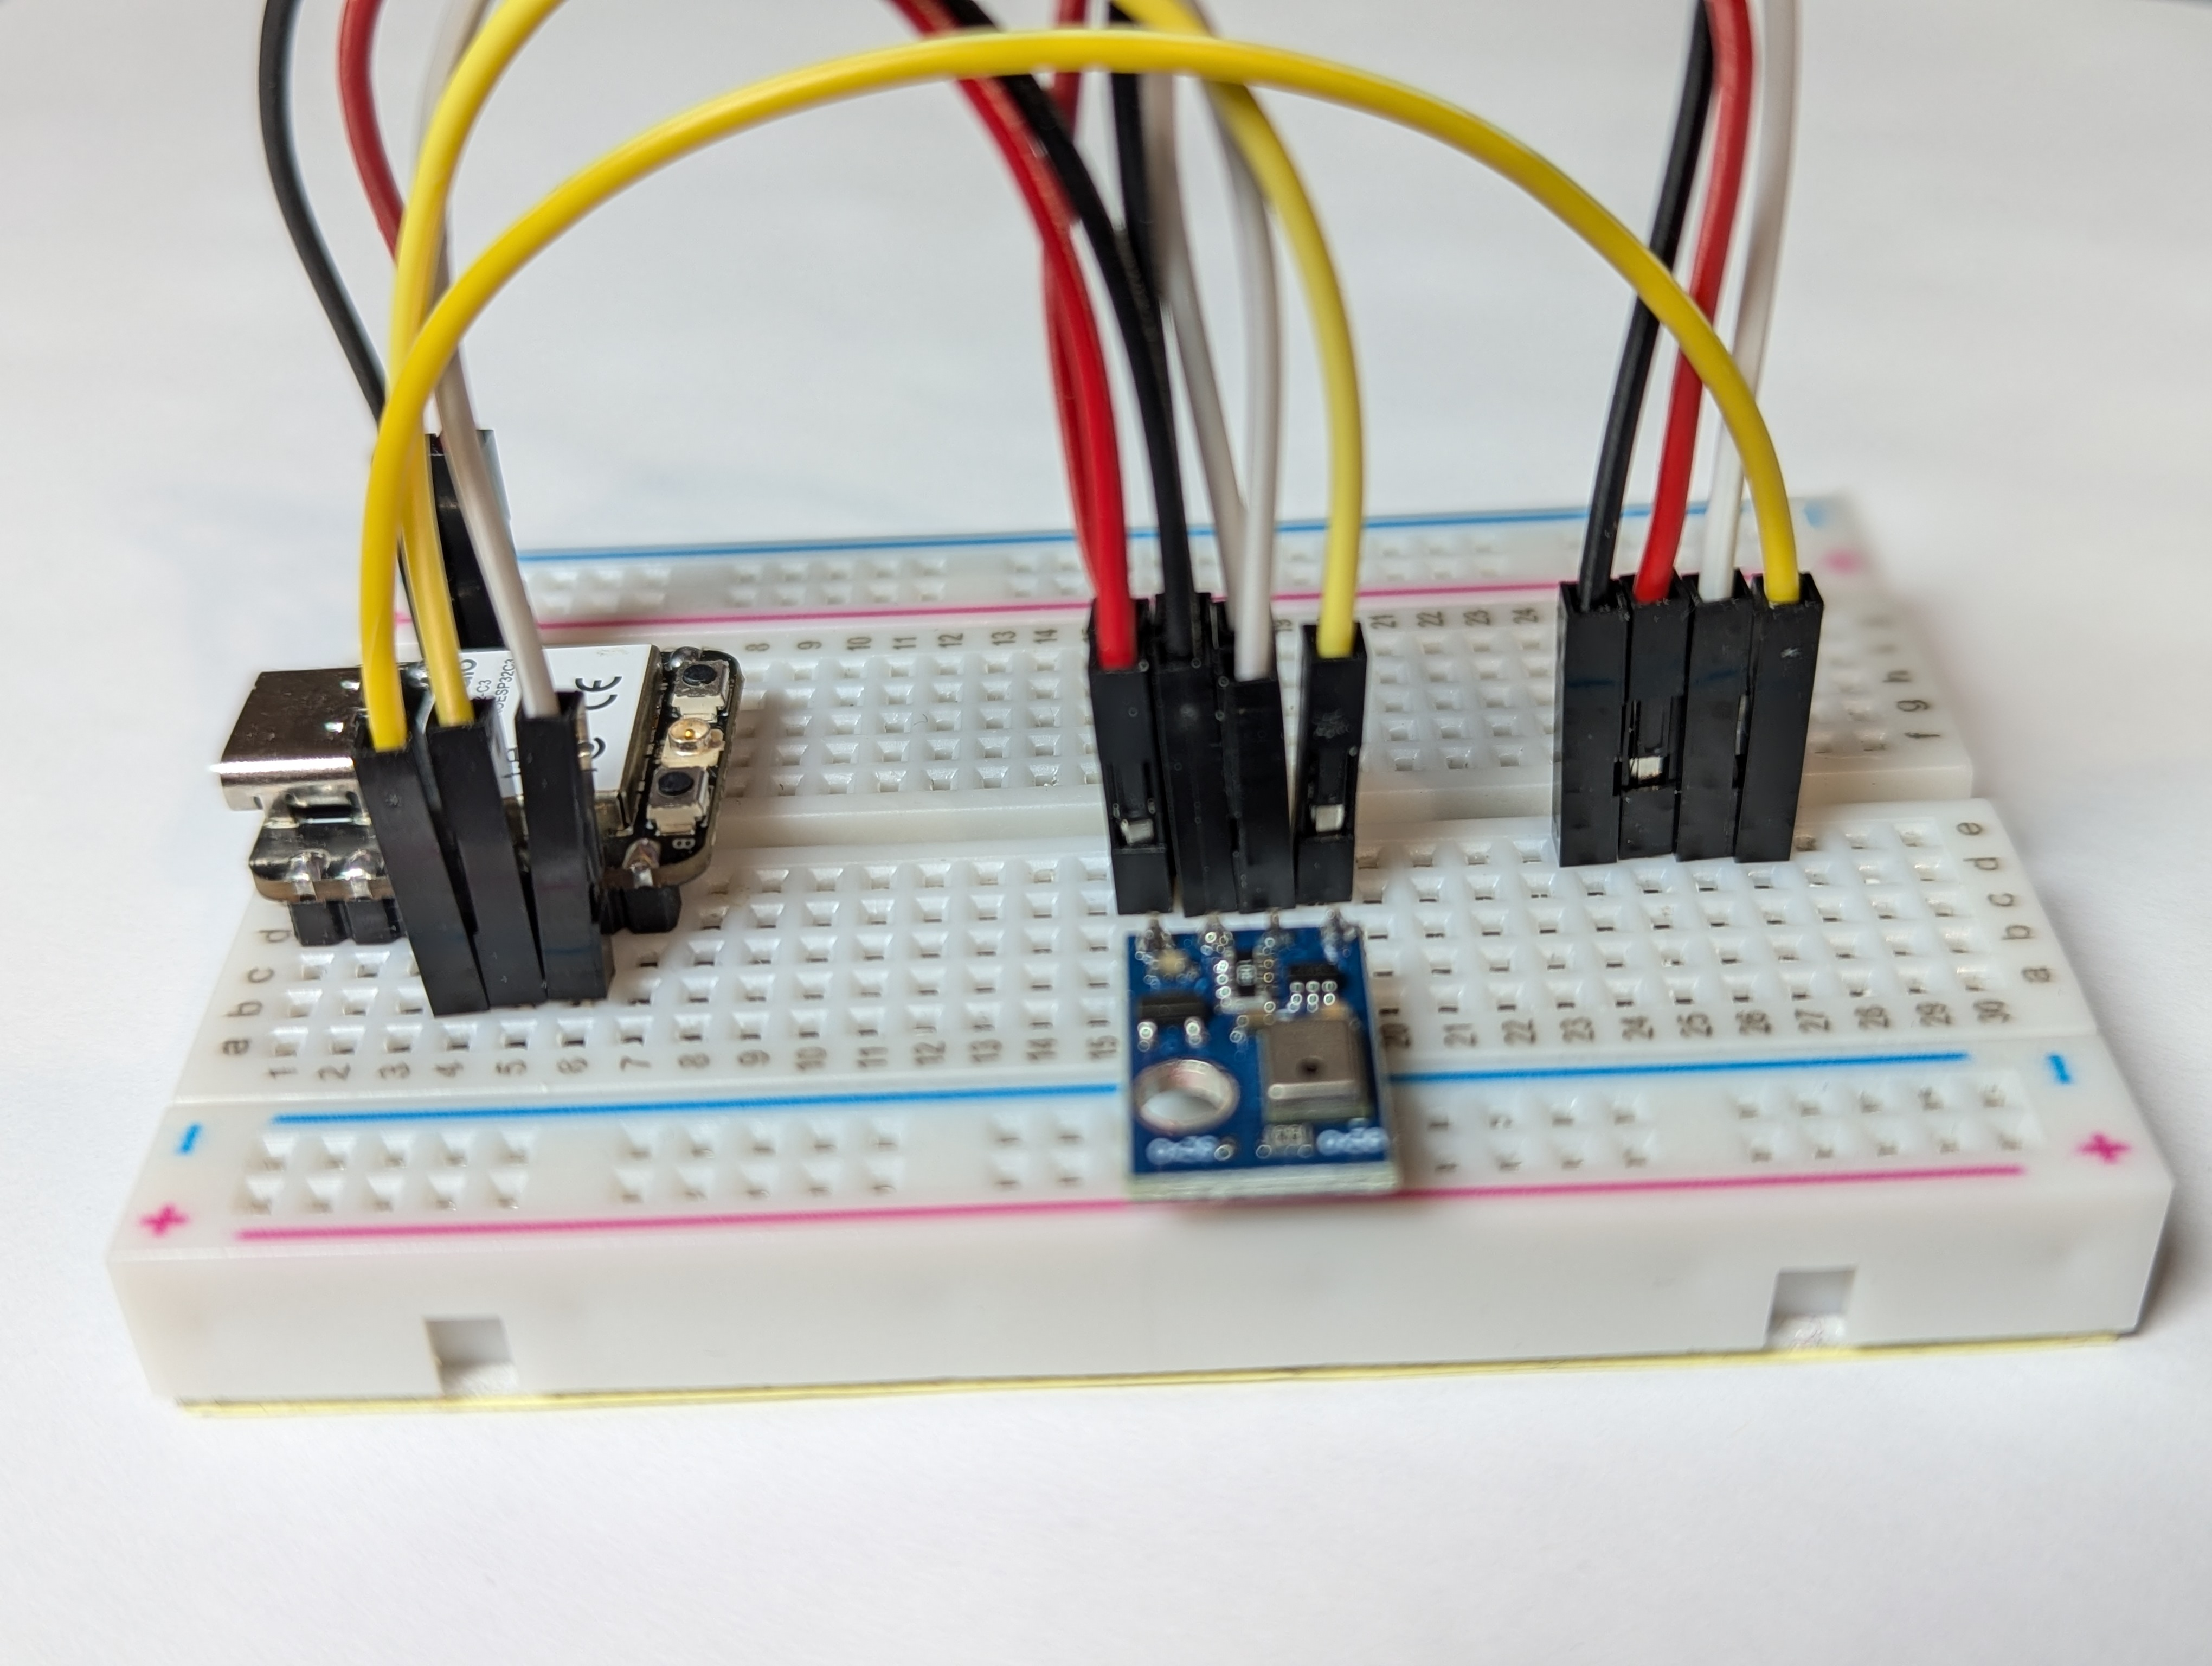
\includegraphics[width=.6\linewidth]{project_4/screen_wired.jpg}
    \caption{The first 3 wires are connected right behind the wires for the sensor. The last wire is connected to the microcontroller.}
\end{figure}

\begin{tcolorbox}[colback=yellow!10!white,colframe=yellow!50!black]
    NOTE: The black and red jumper wires for the temperature sensor are in the reverse order as the
    black and red wires for the screen. If you get them backwards, your microcontroller will not be able
    to power on and it is possible to damage it if you leave it connected for too long.
\end{tcolorbox}

\subsubsection{Attach the screen to the breadboard}
Plug the 4 pins of the screen into the breadboard just under where the 4 new jumper wires are lined up. Make sure the pins of
the screen are lined up with the jumper wires and the screen points away from them. It should look like this:

\begin{figure}[H]
    \centering
    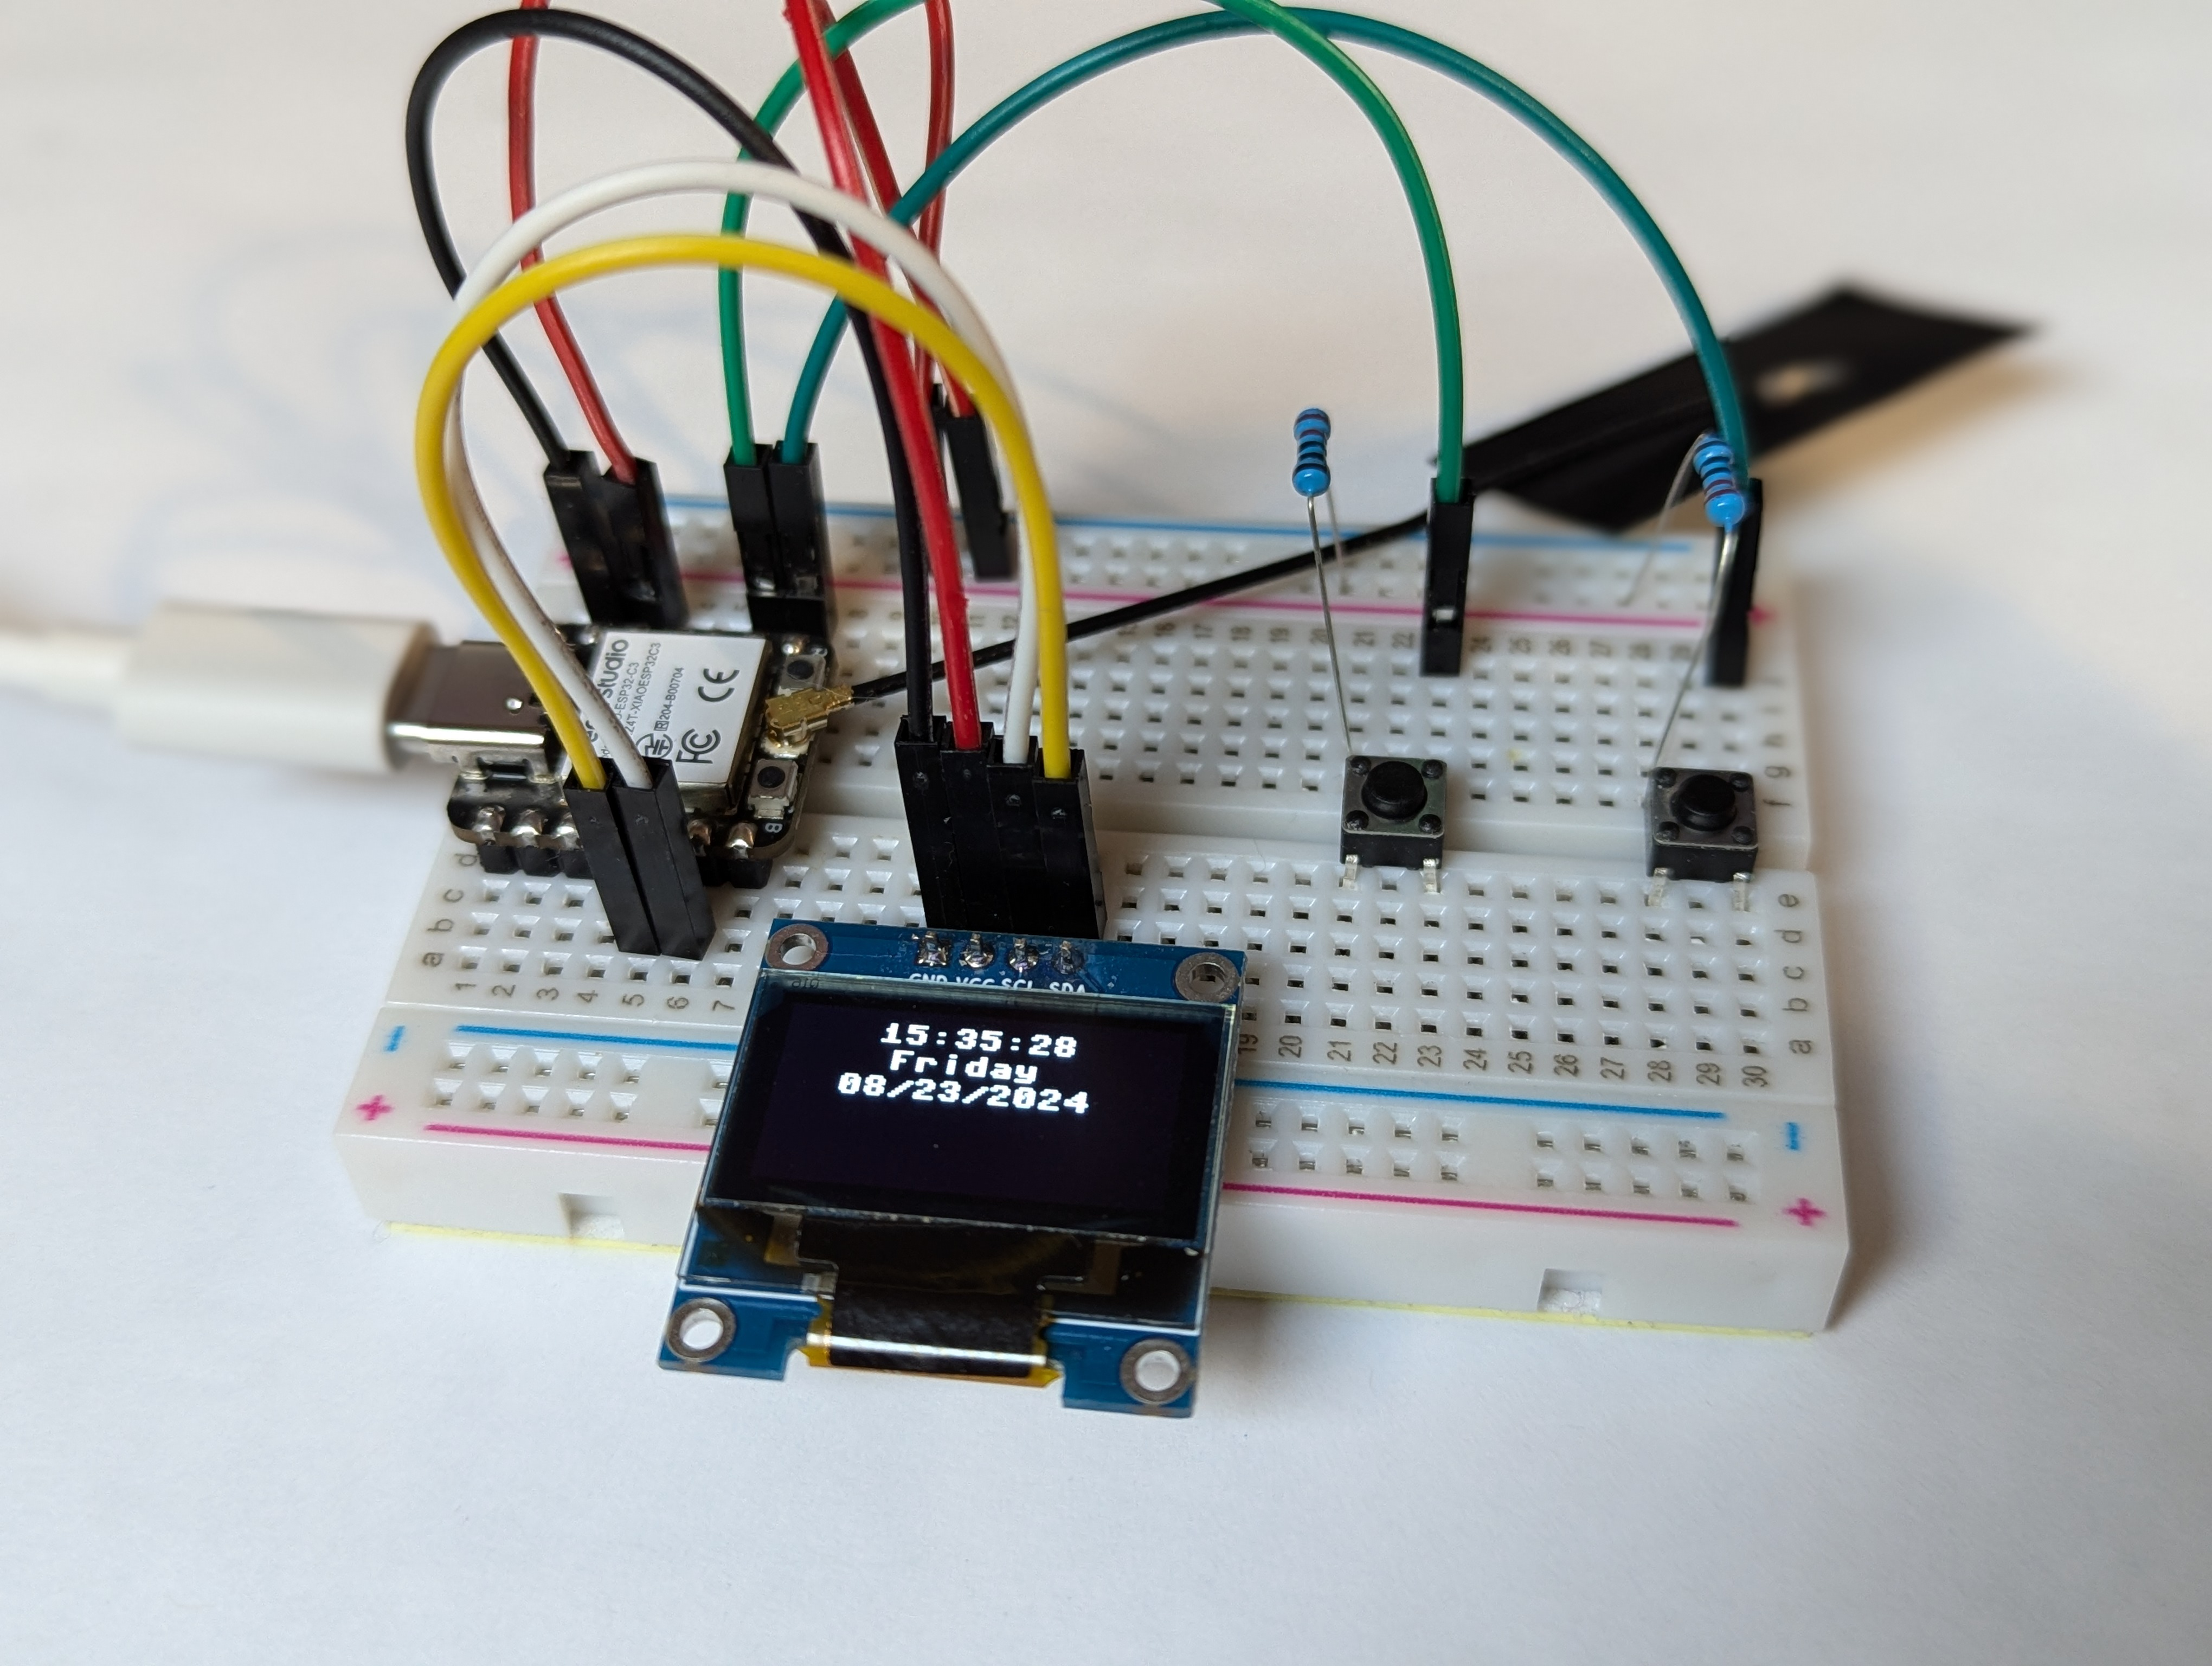
\includegraphics[width=.6\linewidth]{project_4/screen_connected.jpg}
    \caption{Click the button highlighted in red.}
\end{figure}

Plug the USB cable back into the microcontroller and reconnect to it on the IDE interface.
Click on the file named "project\_4b\_sensor.py". This will load the code in the editor for this section. Read through the comments and
the code to get a sense for how it works. Once you are ready, you can click the blue play button in the upper left of the window to start the script:

\begin{figure}[H]
    \centering
    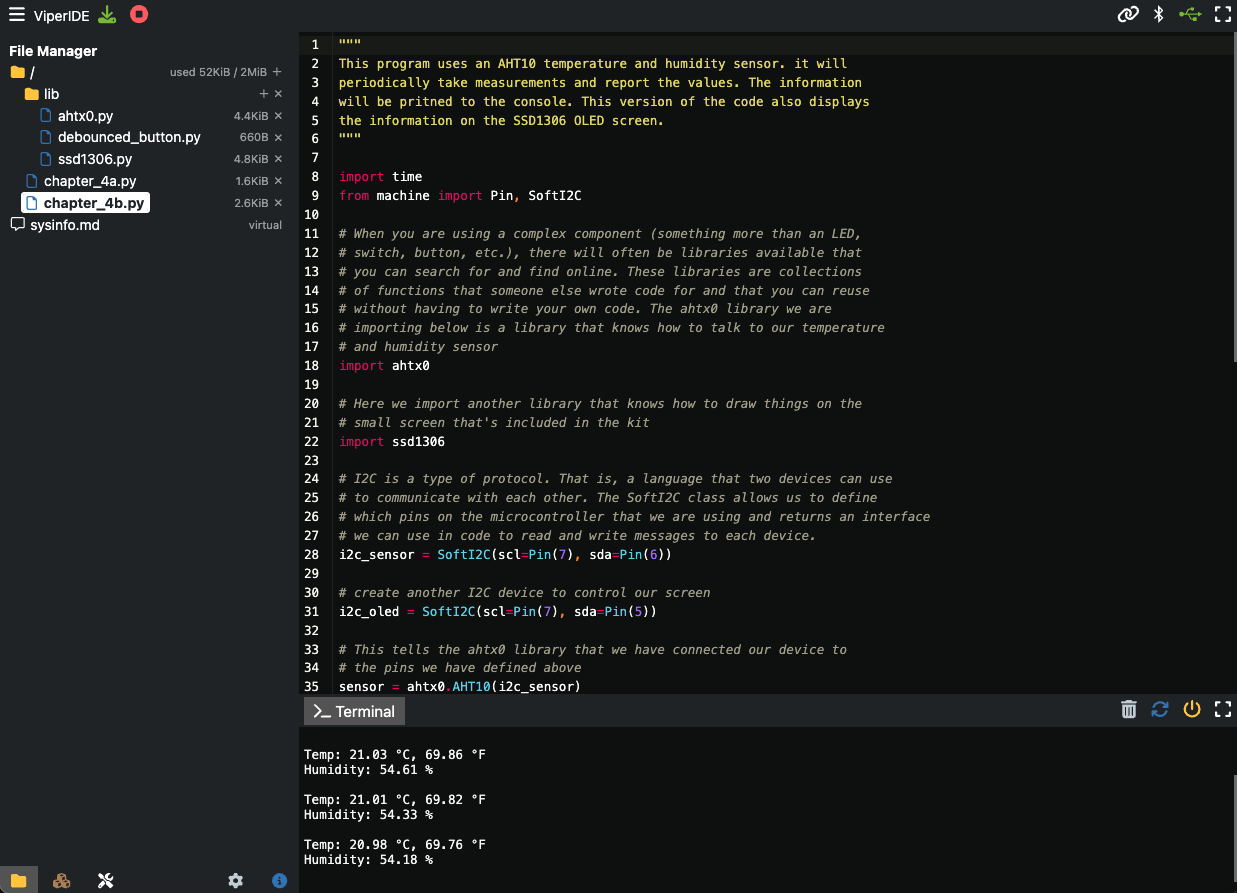
\includegraphics[width=.6\linewidth]{project_4/play_project_4b.png}
    \caption{Once started, this script will run forever and output values into the terminal window and to the OLED screen.
    You can stop by pressing the red stop button.}
\end{figure}

\section{Review}
This project demonstrates how you can connect external sensors to a microcontroller, read their status,
and output that status to a terminal or display. It also demonstrates how you can import external libraries
for talking to these peripheral devices.

\section{Possible Extensions}
If you want to do some experimentation, try these:

\begin{itemize}
    \item Connect an LED and have it light up when the temperature gets warmer than some threshold
    \item Connect a button and have the screen change between several different readouts when pressed
\end{itemize}
